%++++++++++++++++++++++++++++++++++++++++
% Don't modify this section unless you know what you're doing!
\documentclass[letterpaper,12pt]{article}
\usepackage{tabularx} % extra features for tabular environment
\usepackage{amsmath}  % improve math presentation
\usepackage{graphicx} % takes care of graphic including machinery
\usepackage[margin=1in,letterpaper]{geometry} % decreases margins
\usepackage{cite} % takes care of citations
\usepackage[final]{hyperref} % adds hyper links inside the generated pdf file
\hypersetup{
	colorlinks=true,       % false: boxed links; true: colored links
	linkcolor=blue,        % color of internal links
	citecolor=blue,        % color of links to bibliography
	filecolor=magenta,     % color of file links
	urlcolor=blue         
}
\usepackage{tikz}
%++++++++++++++++++++++++++++++++++++++++


\begin{document}

\title{Physical Education 99: Virtual Fitness}
\date{Location: The Big C || Time: 4-7 Fridays }
\author{Instructors: Emily Harari, Loren Curry, Rachel Elia, Melissa Constantino}
\maketitle

\section{General Information}

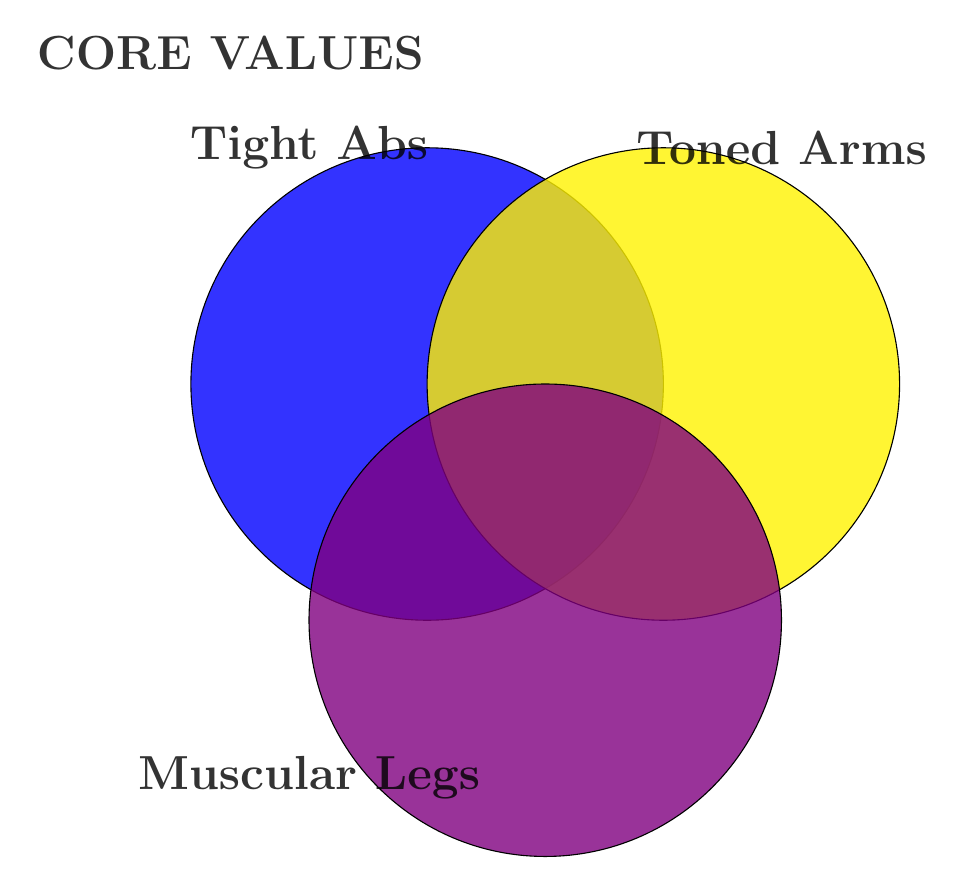
\begin{tikzpicture}
	\begin{scope} [fill opacity = .8]
    \draw[fill=blue, draw = black] (-1.5,1) circle (3);
    \draw[fill=yellow, draw = black] (1.5,1) circle (3);
    \draw[fill=violet, draw = black] (0,-2) circle (3);
    \node at (-4,5.2) {\LARGE\textbf{CORE VALUES}};
    \node at (-3,4) {\LARGE\textbf{Tight Abs}};
    \node at (3,4) {\LARGE\textbf{Toned Arms}};
    \node at (-3,-4) {\LARGE\textbf{Muscular Legs}};
    \end{scope}
    
\end{tikzpicture}


In this DeCal, we will work to improve physical fitness, endurance, and respiratory strength through fun and engaging workouts. Our daily warm up will be the walk to the top of the Big C, and from there we will engage in different workout programs such as Just Dance, Wii Sports, and other virtual fitness games and programs. Students will learn a variety of fitness techniques in class that they can apply to their everyday fitness schedule. By the end of this course, students will have a large knowledge of workouts to improve their own fitness, as is the goal of the Physical Education program at UC Berkeley.  

Emily's office hours: M, W 2-3 PM at Memorial Glade. Loren: T, Th 5-6 AM at Free Speech Movement Cafe. Rachel: Th, F 1-3 PM at Faculty Glade. Melissa: T, W 5-7 PM at Pat Brown's Cafe.


\section{Course Requirements and Policies}

All students must have a fun and positive attitude toward trying new things. There are no prior pre-requisites necessary to take this course. There is one required reading which will help to build on the information covered in the class. The material from the book will be included in the final physical test.\\
\\
Required Reading: The 4-Hour Body by Tim Ferriss \\
\\
Attendance will be measured via role call. Each lecture counts for 3 points. 15\%\ of the  of the total assignment grade will be deducted for every day it is turned in late. Plagiarism will not be tolerated. Any evidence of cheating will result in immediately failure in the course.

\section{Office Hours}
It is highly encouraged that students attend office hours. This time is crucial for students to ask questions on subjects they struggle with, expand their knowledge, and get to know the instructors. They are crucial for the success in this course. 




\section{Grading}
\begin{table}[ht]
\begin{center}
\caption{Grade Distribution}
\label{tbl:bins} % spaces are big no-no withing labels
\begin{tabular}{|cc|} 
\hline
\multicolumn{1}{|c}{Assignments} & \multicolumn{1}{c|}{Weight} \\
\hline
Attendance &   30\% : 30 points \\
Participation and Enthusiasm &   20\%: 40 points \\
Workout Project &   25\% : 40 points \\
Physical Test &  25\% : 40 points \\
\hline
\end{tabular}
\end{center}
\end{table}

This class is 2 units, P/NP only. 105+/150 points is required to pass the course.   Attendance is worth 30\%\ of the overall grade. There will be one project worth 35 points. Participation and visible enthusiasm is worth 35 points. A physical test at the end of the semester is worth 35 points.

All grades will be uploaded to bcourses, so that students may know their progress in the class. Additional surveys will be sent out during the semester to gain feedback from students on the course.
\\
\\
\\
\section{Calendar}
\begin{table}[ht]
\begin{center}
\caption{Course Schedule}
\label{tbl:bins} % spaces are big no-no withing labels
\begin{tabular}{|cc|} 
\hline
\multicolumn{1}{|c}{DATE} & \multicolumn{1}{c|}{TOPIC} \\
\hline
8/31/18 &   Introduction                      \\
9/7/18 &   Just Dance on the Wii \\
9/14/18 &   Wii Sports: Step Dance \\
9/21/18 &   Wii Sports: Tennis \\
9/28/18 &   Wii Sports:  Boxing\\
10/5/18 &   Guest Speaker - Jillian Michaels \\
10/12/18 &   Wii Fit: Boxing \\
10/19/18 &   Wii Fit: Hula-Hooping \\
10/26/18 &   Wii Fit: Yoga \\
11/2/18 &   Wii: Zumba Fitness \\
11/9/18 &   Xbox Kinect: Get Fit with Mel B  \\
11/16/18 &   Final Project Due  \\
11/23/18 &   Thanksgiving Break -- No Class \\
11/30/18 &   Physical Fitness Test \\
\hline
\end{tabular}
\end{center}
\end{table}



\end{document}
